Digital image processing is a field of computer vision that deals with the manipulation, analysis, and interpretation of digital images. It focuses on algorithms and techniques that extract meaningful information from images and to enhance visual quality. In fluoroscopy, image processing can be used to enhance the digital image, or determine important information about it such that a the model-image registration task can be performed efficiently and autonomously.

\subsubsection{Filtering and Convolution}
\label{sec:filtering-convolution}
We have already seen how image formation yields a collection of 2D points, $\mathbf{x}_{pix}$. We can write the intensity values at each pixel locations as a function, $f(\mathbf{x}_{pix}) = f(i,j)$, where $(i,j)$ represent locations in the image, and the function returns the intensity of the image at that particular pixel location. This allows us to treat images as functions, and perform similar functional operations and analysis to extract meaningful information from them.

The most widely used filter is a linear filter \cite{szeliskiComputerVisionAlgorithms2022}, where the output is some linear operation on the neighboring pixels (Eq. \ref{eq:convolution}), also known as a \emph{convolution}. In a convolution, the kernel, $h$ is shifted along the input image, $f$, and the resultant image, $g$, is the dot product of those two matrices at that specific location.

\begin{equation}
    \begin{aligned}
        g(i,j) &= \sum_{k,l}f(i-k,j-l)h(k,l) \\
        &= \sum_{k,l}f(k,l)h(i-k,j-l) \\
        &\text{Where we use the following notation}\\
        g&= f * h
    \end{aligned}
    \label{eq:convolution}
\end{equation}

The convolution operation is \emph{linear shift invariant}, which means that it obeys the superposition principle (Eq. \ref{eq:superposition}) and the shift invariance principle (Eq. \ref{eq:shift-invariance}). This is a powerful property, because it will behave the same everywhere on the input signal/image, which is useful for different types of feature extraction and filtering operations.

\begin{equation}
    h *(f + g) = h*f + h*g
    \label{eq:superposition}
\end{equation}

\begin{equation}
    g(i,j) = f(i+k,j+l) \Longleftrightarrow (h*g)(i,j) = (h*f)(i+k,j+l)
    \label{eq:shift-invariance}
\end{equation}

A common filter applied to images is the Gaussian kernel (Eq. \ref{eq:gaussian-kernal}). This kernel is shaped as a 2D discrete Gaussian, and has the effect of blurring an image and removing noise.

\begin{equation}
    \text{Gaussian filter}=\frac{1}{256}\begin{bmatrix}
        1 & 4 & 6 & 4 & 1 \\
        4 & 16 & 24 & 16 & 4\\
        6 & 24 & 36 & 24 & 6\\
        4 & 16 & 24 & 16 & 4\\
        1 & 4 & 6 & 4 & 1 \\
    \end{bmatrix}
    \label{eq:gaussian-kernal}
\end{equation}

Another is the box kernel, which averages the value of the nearest K pixels (Eq. \ref{eq:box-filter}).

\begin{equation}
    \text{Box filter} = \frac{1}{K^{2}}\begin{bmatrix}
        1 & 1 & \cdots &1\\
        1 & 1 & \cdots &1 \\
        \vdots & \vdots & 1 & \vdots \\
        1 & 1 & \cdots & 1
    \end{bmatrix}
    \label{eq:box-filter}
\end{equation}

Edge filters can also be created to detect vertical (Eq. \ref{eq:vert-edge-filter}), horizontal (Eq. \ref{eq:horiz-edge-filter}), or diagonal edges (Eq. \ref{eq:diag-edge-filter}). As each of the filters moves across the feature it is designed for, that region of the output will be more highly activated than other regions, extracting out the desired components. The orientation of each of these filters can be hand-selected to find desirable attributes in images.

\begin{equation}
    \text{vertical edge filter} = \begin{bmatrix}
            0 & 1 & 0 \\
            0 & 1 & 0 \\
            0 & 1 & 0 \\
    \end{bmatrix}
    \label{eq:vert-edge-filter}
\end{equation}

\begin{equation}
    \text{horizontal edge filter} =\begin{bmatrix}
        0 & 0 & 0 \\
        1 & 1 & 1 \\
        0 & 0 & 0 \\
    \end{bmatrix}
    \label{eq:horiz-edge-filter}
\end{equation}

\begin{equation}
    \begin{aligned}
        \text{diagonal edge filters} = \begin{bmatrix}
            1 & 0 & 0 \\
            0 & 1 & 0\\
            0 & 0 & 1
        \end{bmatrix}& \text{and} & 
        \begin{bmatrix}
            0 & 0 & 1 \\
            0 & 1 & 0\\
            1 & 0 & 0
        \end{bmatrix}
    \end{aligned}
    \label{eq:diag-edge-filter}
\end{equation}

Lastly, we can use a corner filter to find corners in images (Eq. \ref{eq:corner-filter}).

\begin{equation}
    \text{Corner filter} = \frac{1}{4}\begin{bmatrix}
        1 & -2 & 1 \\
        -2 & 4 & -2 \\
        1 & -2 & 1 \\
    \end{bmatrix}
    \label{eq:corner-filter}
\end{equation}

Entire subfields of computer vision and image analysis are devoted to creating increasingly useful and complex filters, or collections of filters. These include steerable filters, which determine information occurring in arbitrary directions \cite{freemanSteerableFiltersLocal1992}, recursive filtering \cite{nielsenRegularizationScalespaceEdge1996}, and non-linear filtering \cite{tomasiBilateralFilteringGray1998}.

\subsubsection{Binary Image Processing}
\label{sec:binary-img-proc}

A binary image is a digital image that consists only of black and white pixels. It is often used for labeling or masking an underlying image, where the values of 1 and 0 represent the presence or absence of a particular feature or object. Binary images are often used in computer vision and image processing applications because they can be easily processed and analyzed using algorithms. They are also useful for storing and transmitting large amounts of data, as the use of only two values reduces the amount of information that needs to be stored and transmitted.

The primary form of processing on binary images is morphological, that is, changing the shape of the ``blob'' in order to extract useful information from it.

\begin{figure}[h!]
    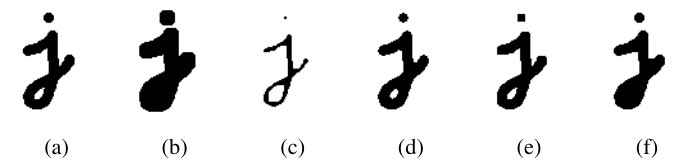
\includegraphics[width = \linewidth]{figs/background/png/binary-image-processing.jpg}
    \caption{A collection of morphological operations on a binary image: (a) original image; (b) dilation; (c) erosion; (d) majority; (e) opening; (f) closing. Image from \cite{szeliskiComputerVisionAlgorithms2022}}
    \label{fig:binary-image-processing}
\end{figure}

Dilation and erosion are the two main operations that are used in model-image registration (\ref{eq:dilation-erosion}). These functions are ach two-fold: first, a convolution operation is applied to the existing binary image, then a threshold is applied to the convolution output to determine if the central pixel is a zero or 1. If $f$ is the input image, $s$ is the convolution kernel of $1$s, and $c=f\otimes s$ is the number of $1$s in the convolution output, then dilation and erosion can be expressed in the following way.

\begin{equation}
    \begin{aligned}
        \text{dilate}(f,s) &= \theta(c,1) \\
        \text{erode}(f,s) &= \theta(c,S) 
    \end{aligned}
    \label{eq:dilation-erosion}
\end{equation}

Where $\theta$ represents a thresholding function.

\begin{equation}
    \theta (f,t) = \begin{cases}
        1 &\text{ if } f\ge t \\
        0 &\text{ else}
    \end{cases}
\end{equation}